\subsection{Collision Detection for Rotated Objects}
The user should be able to select the object by clicking inside of the hitbox, even when the object is rotated.
This gave an issue when rotating an object the hitbox did not follow and to click on the object you had to click inside the misplaced hitbox.

The reason for this was that when the object was created the hitbox was set but never changed after rotating the object.
Therefore, a change was made to the hitbox property such that the top left corner of the hitbox was set to the minimum x and y value of an objects coordinates.

To find the new points of the rotated object we used the rotation matrix to rotate the current corners of the object.
As seen in \lstref{lst:changeHitbox} the minimum x and y values of these corners are then found, and used to find the top left corner of the hitbox.
Once this corner has been found, the width and height can be calculated by using the corner and the center of the object.

In \figref{figure:hitbox} the hitbox can be seen around the hitbox both when rotated and not rotated.

\begin{lstlisting}[caption={Method to change the hitbox},label=lst:changeHitbox]
protected void changeHitbox(){
	FloatPoint one = rotationMatrix( -(getWidth()/2), -(getHeight()/2));
	FloatPoint two = rotationMatrix((getWidth()/2), -(getHeight()/2));
	FloatPoint three = rotationMatrix((getWidth()/2), (getHeight()/2));
	FloatPoint four = rotationMatrix( -(getWidth()/2), (getHeight()/2));
	
	hitboxTopLeft = new FloatPoint(
	    findMin(one.x, two.x, three.x, four.x),
	    findMin(one.y, two.y, three.y, four.y));
	hitboxWidth = (getCenter().x - hitboxTopLeft.x)*2;
	hitboxHeigth = (getCenter().y - hitboxTopLeft.y)*2;
}
\end{lstlisting}



\begin{figure}[h]
	\centering
	%---- linebreak	
	\begin{subfigure}[b]{0.45\textwidth}
		\centering
		\includegraphics[scale = 0.3]{sprint1/rectangle}
		\caption{Hitbox for standard rectangle}
		\label{figure:hitbox-rectangle}
	\end{subfigure}
	\qquad
	\begin{subfigure}[b]{0.45\textwidth}
		\centering
		\includegraphics[scale = 0.3]{sprint1/rectangle-rotated}
		\caption{Hitbox for a rotated rectangle.}
		\label{figure:hitbox-rotated-rectangle}
	\end{subfigure}
	\caption{The different hitboxes.}
	\label{figure:hitbox}
\end{figure}

A new issue that emerged was that the collision detection for the object was now larger than the object.
When an object was behind a rotated object, and the user clicked the in the top left corner of the hitbox, the rotated object would be selected instead of the object behind.
To resolve this issue, an implementation was done to give a precise collision detection on the object, which will be described below.

\subsubsection{Precise Collision Detection for Rotated Rectangles}
To understand the mathematics behind the precise collision detection for rotated rectangles, an illustration of the problem can be seen in \figref{figure:rectangle-collision}.

\begin{figure}[h]
	\centering
	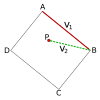
\includegraphics[scale=2]{sprint1/rectangle-collision}
	\caption{Vectors showing a right rotation.}
	\label{figure:rectangle-collision}
\end{figure}

The idea behind the mathematical formula is to see whether the vector to the point is a right rotation of all the rectangle's sides.
To determine this we compare the slope of the vectors.
The formula to determine a right rotation is:
\begin{equation}
	\frac{B_x-A_x}{B_y-A_y} \geq \frac{P_x-B_x}{P_y-B_y}
\end{equation}

The formula is changed to avoid divide by zero errors, and is therefore changed to the following equation:
\begin{equation}
	(B_x-A_x)*(P_y-B_y) \geq (P_x-B_x)*(B_y-A_y)
\end{equation} 

\subsubsection{Precise Collision Detection for Rotated Ellipses}


\subsubsection{Precise Collision Detection for Rotated Lines}

\begin{figure}[h]
	\centering
	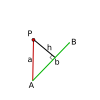
\includegraphics[scale=2]{sprint1/line-collision}
	\caption{Drawing showing the idea behind the mathematical formula.}
	\label{figure:line-collision}
\end{figure}

\begin{equation}
	A = \frac{1}{2}*h*G
\end{equation}

\begin{equation}
	A =  \frac{1}{2}*|\vec{a} \times \vec{b}|
\end{equation}

\begin{equation}
\begin{aligned}
	\frac{1}{2}*h*G &=  \frac{1}{2}*|\vec{a} \times \vec{b}|\\
	& \Downarrow \\
	h &=  \frac{|\vec{a} \times \vec{b}|}{G}
\end{aligned}
\end{equation}

\begin{equation*}
	|\vec{b}| = G
\end{equation*}

\begin{equation}
	|\vec{a} \times \vec{b}| = 
	\begin{bmatrix}
		P_x-A_x \\
		P_y-A_y
	\end{bmatrix}
	\times
	\begin{bmatrix}
		B_x-A_x \\
		B_y-A_y
	\end{bmatrix}
\end{equation}

\begin{equation}
\begin{aligned}
	h &= \frac{|\vec{a} \times \vec{b}|}{|\vec{b}|}\\
	  &= \frac{|(P_x-A_x)(B_y-A_y)-(P_y-A-y)(B_x-A_x)|}{\sqrt{b_x^2+b_y^2}}\\
	  &= \frac{|P_xB_y-P_xA_y-A_xB_y-P_yB_x+P_yA_x+A_yB_x|}{\sqrt{b_x^2+b_y^2}}
\end{aligned}
\end{equation}







